\section{Stato dell'Arte}

\subsection{Modelli Compartimentali}
In epidemiologia i modelli compartimentali sono una tecnica di modellezione 
generica che si predispone molto bene allo studio complessivo del comportamento
di una malattia infettiva \cite{wiki:Compartmental_models_in_epidemiology}. 
Questa tecnica di modellazione si applica anche ad altre branche della 
scienza, come ad esempio la finanza.

Questa tecnica di modellazione matematica basa il proprio funzionamento 
sull'assunzione che, data una popolazione di individui, questi vengano 
etichettati in maniera differente, in base allo stato di progressione 
della malattia che hanno, o non hanno, contratto. Così facendo si vanno a 
definire dei compartimenti ben separati che possono interagire tra loro, ma 
che rimangono comunque chiaramente distinti l'uni dagli altri.

Il modello che tutt'ora viene usato come riferimento e come base per 
lo studio e modellazione è il così detto modello SIR: Susceptible, Infectious, Recovered.

\begin{figure}[h]
    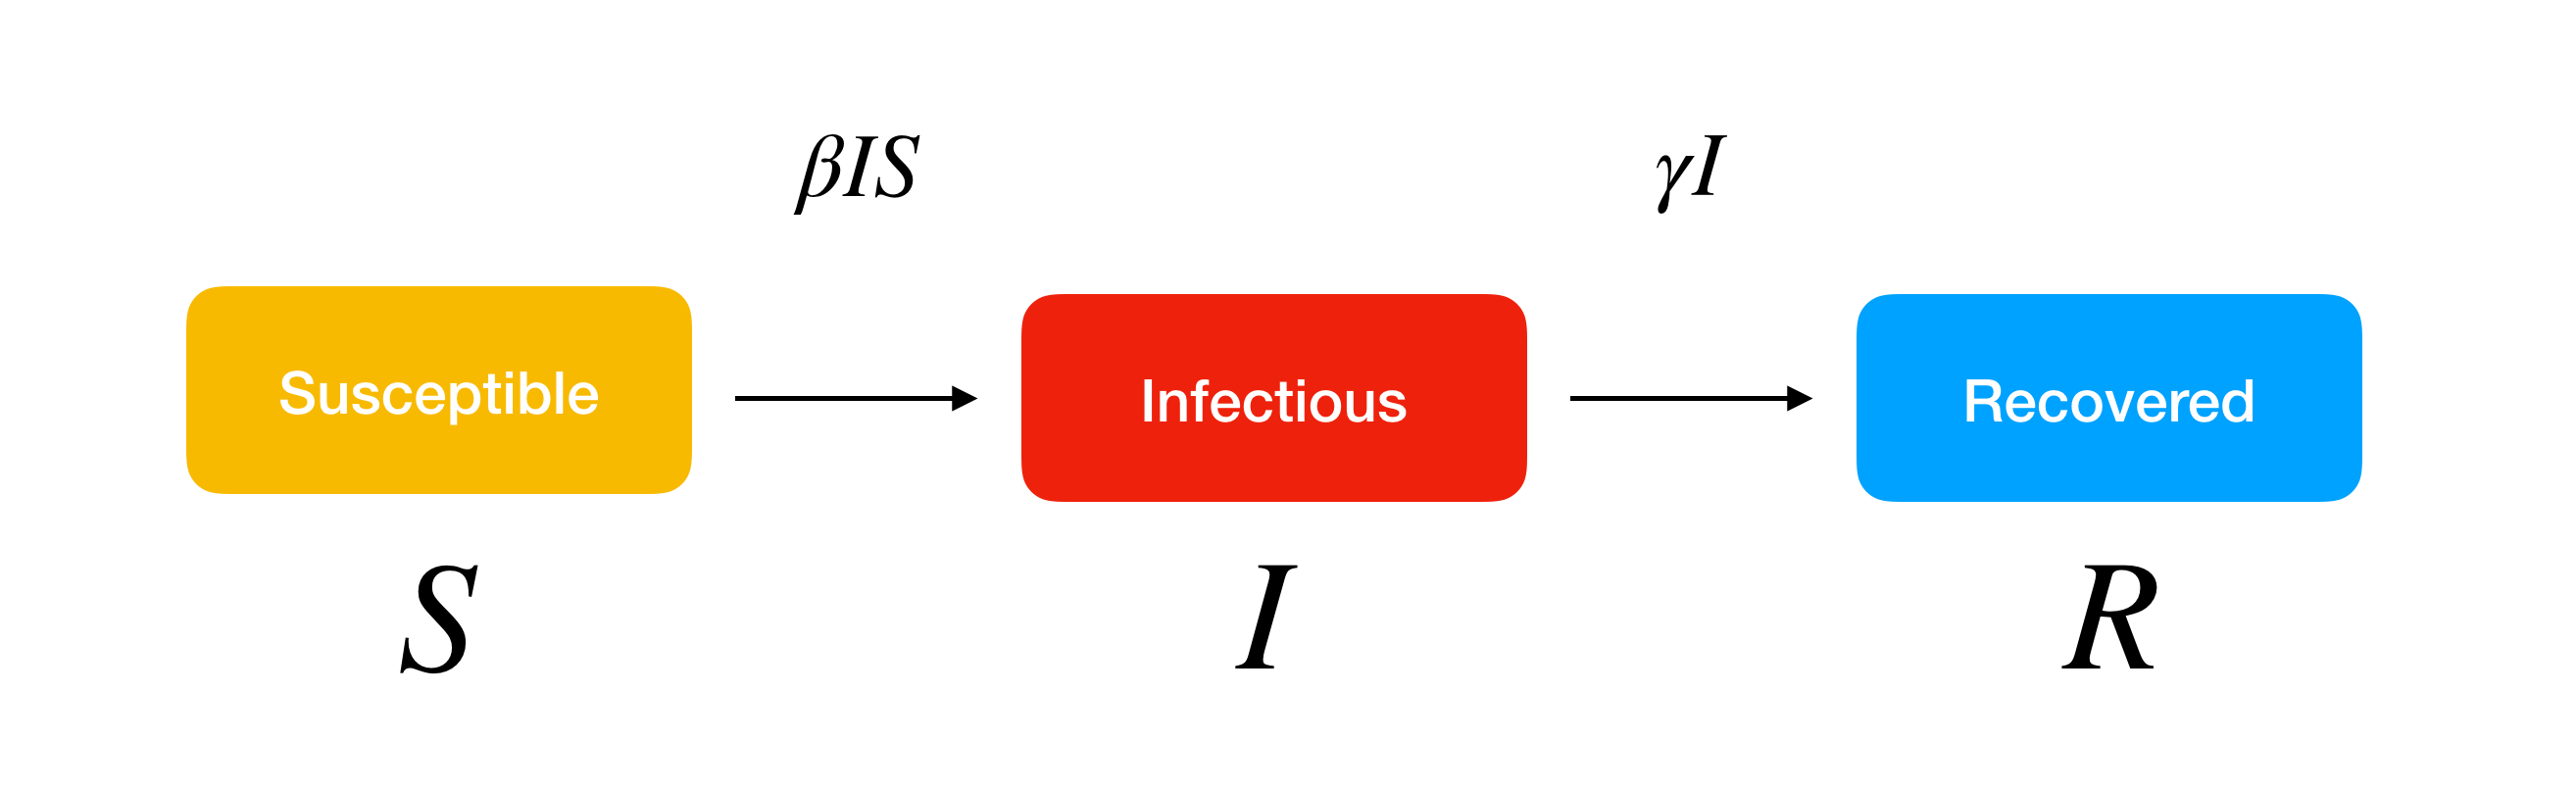
\includegraphics[width=\linewidth]{img/sir.png}
    \caption{Struttura modello SIR} 
    \label{fig:SIR_Structure}
\end{figure}

Questo modello è stato ideato all'inizio del 20esimo secolo, 
più precisamente nel 1917, da Kermack e McKendrick. Come introdotto questo modello
si basa sull'assunzione che all'interno di una popolazione durante 
il decorso di una malattia vi possano esistere solamente tre stadi in cui 
un individuo può essere inserito: 

\begin{itemize}
    \item Susceptible: Questo stadio rappresenta lo stato iniziale per la maggior parte
    degli individui all'interno di una popolazione. Rappresenta il numero di 
    persone che possono contrarre la malattia.
    \item Infectious: Questo stadio rappresenta tutti quegli individui che dallo 
    stato di Susceptible, dopo essere venuti in contatto con un individui infetto, 
    diventano a loro volta individui infetti.
    \item Recovered: Questo stadio rappresenta una duplice categoria, quella degli
    individui che alla fine del docorso della malattia sopravvivono ad essa, e 
    quelli che invece muoiono a causa di questa. Generalemente questo stato viene
    anche definito come Removed.
\end{itemize}

\newpage

\begin{figure}[h]
    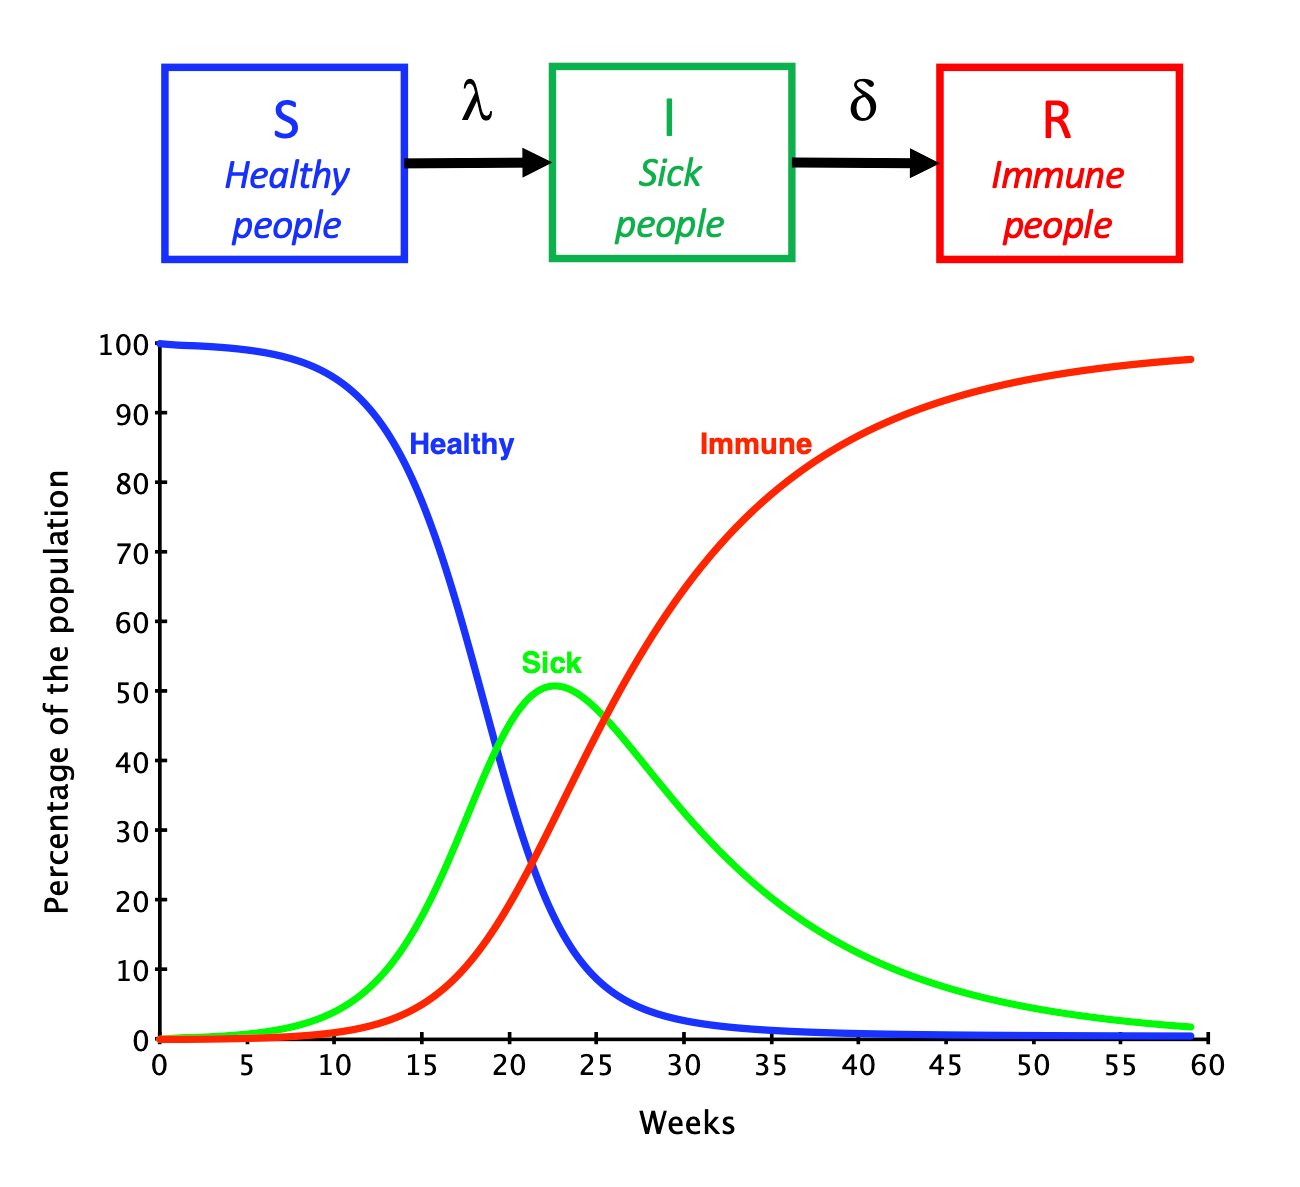
\includegraphics[width=\linewidth]{img/SIR-model.png}
    \caption{Visualizzazione grafico modello SIR} 
    \label{fig:SIR_model_graphic}
\end{figure}

Questo semplice modello funziona grazie all'utilizzo di un sistema di Equazioni
Ordinarie Differenziali (ODE) \cite{Brauer2008}. Una volta definiti i parametri iniziali 
utili per la simulazione del decorso di una malattia, è pressocchè immediato trovare
il risultato al tempo T del sistema. Questo modello può essere calcolato tenendo 
in considerazione un andamento più caotico del sistema, utilizzando invece che 
un sistema di ODE, un sistema di SDE \cite{Allen2008} ovvero di Equazioni Differenziali Stocastiche.

% \begin{figure}[h]
%    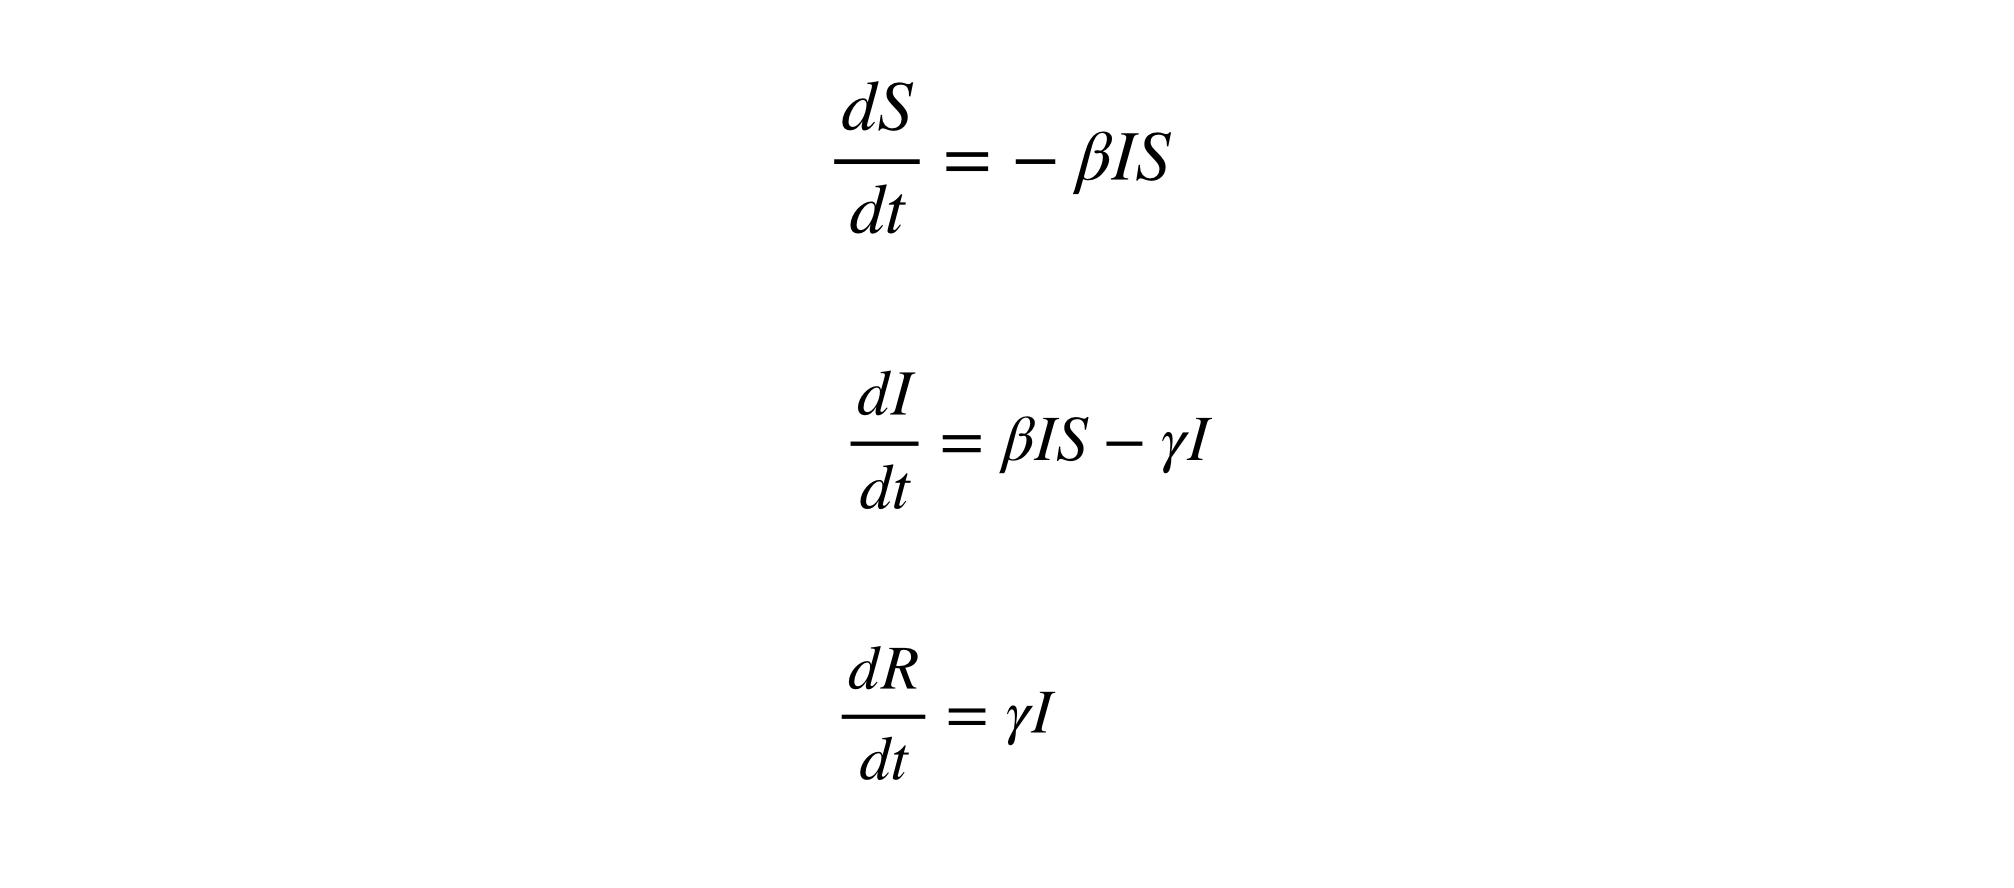
\includegraphics[width=\linewidth]{img/ode.png}
%    \caption{Equazioni Ordinarie Differenziali modello SIR} 
%    \label{fig:ODE_SIR}
% \end{figure}

Con il tempo questo sistema è stato espanso per tenere in considerazione comportamenti
differenti sia della popolazione che delle malattie, andando a definire una moltitudine
di modelli utili a differenti scopi. In epidemiologia il modello di
riferimento maggiormente utilizzato è il modello SEIR (Susceptible, Exposed, Infectious, Recovered)
con le sue varianti proprie di ogni approccio.

Alcuni modelli definiscono i propri stati in maniera da considerare 
come stato interno al sistema anche l'agente patogeno, così da 
poter modellare e simulare l'andamento dell'infettività della pandemia 
in relazione alle contromisure prese, siano esse farmaceutiche o non.
Ne è un esempio il modello proposto da \cite{Mwalili2020} nel quale 
il modello viene proposto con l'idea di incorporare le misure di 
distanziamento sociale come variabili per misurare la loro efficacia
contro la recente pandemia da COVID-19.

\begin{figure}[h]
    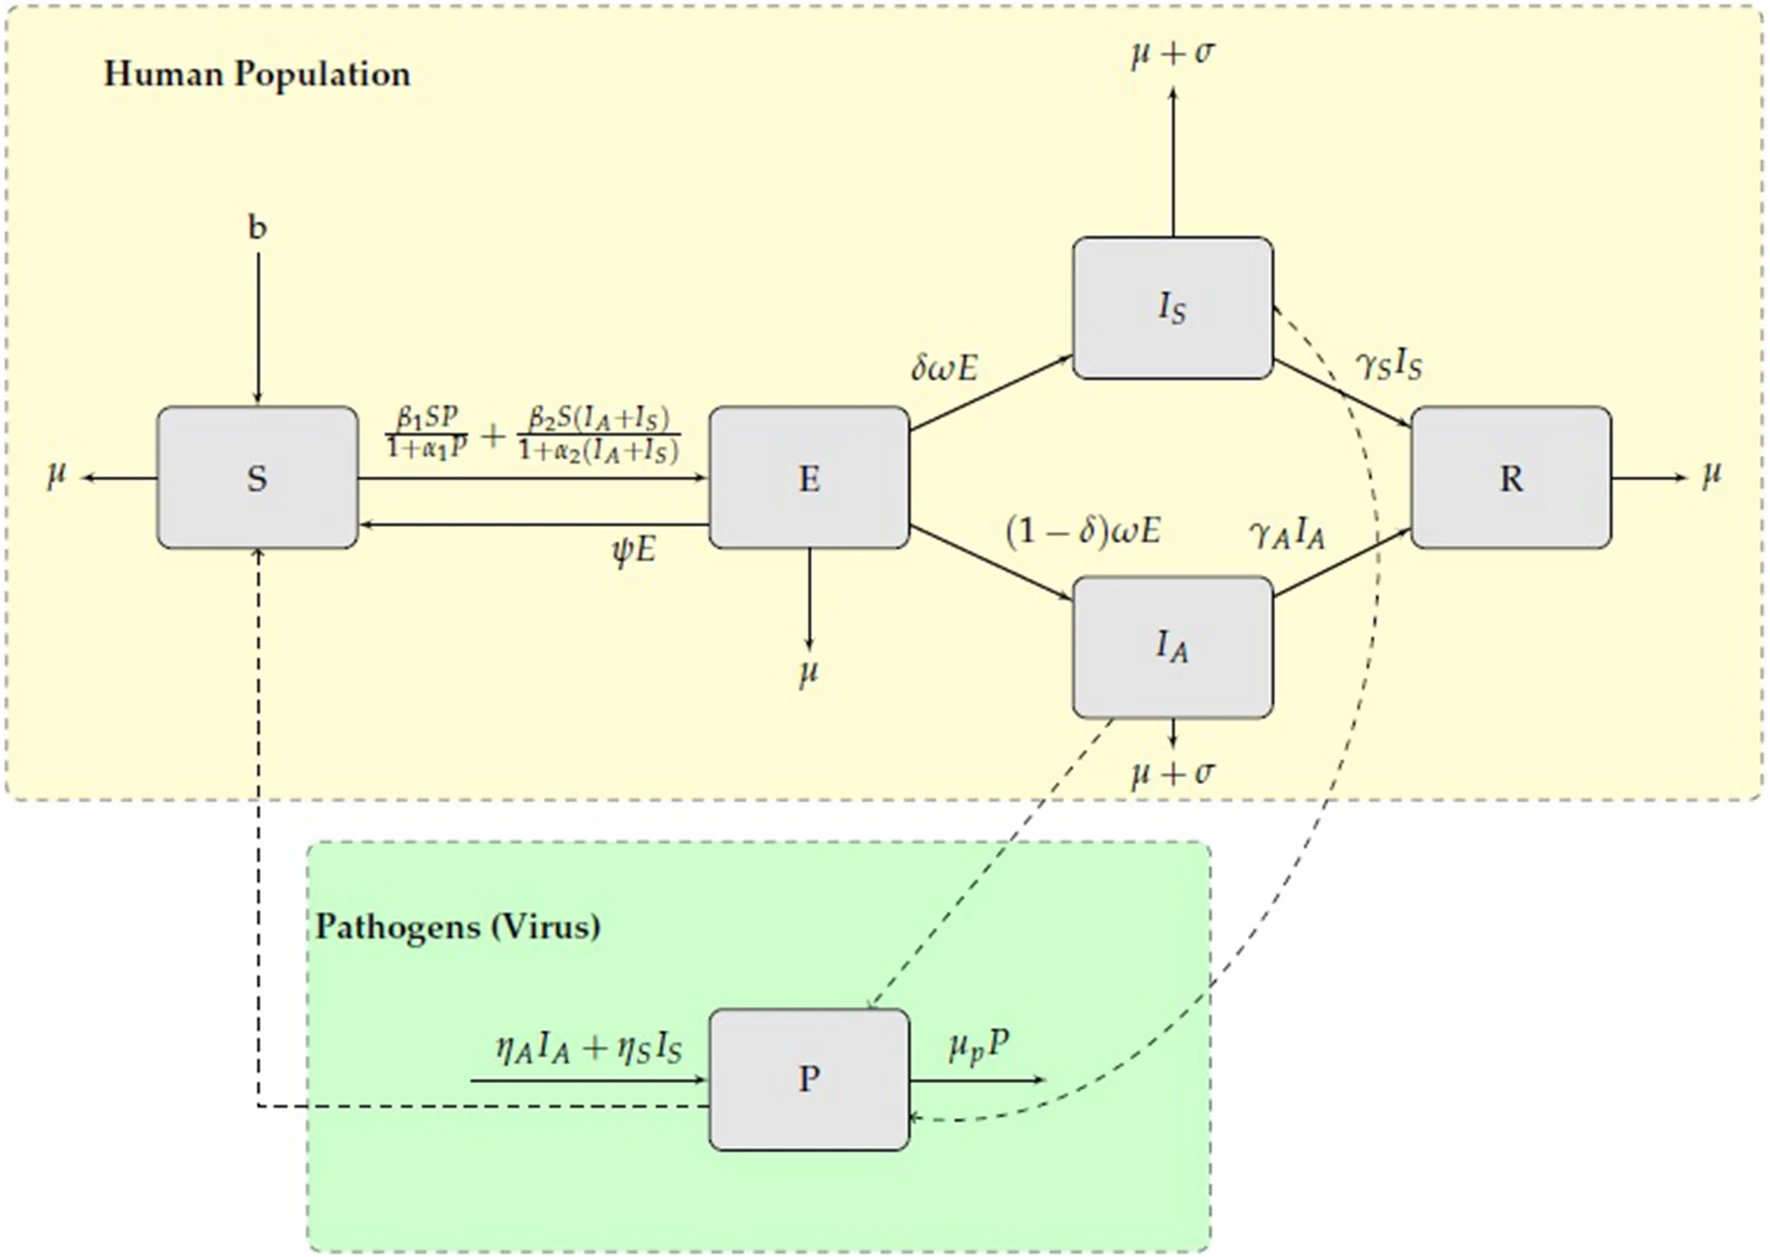
\includegraphics[width=\linewidth]{img/13104_2020_5192_Fig1_HTML.png}
    \caption{Esempio di modello SEIR preso dall'articolo \cite{Mwalili2020}}
    \label{fig:SEIR_model_social_distancing}
\end{figure}

Altri modelli, come quello proposto da \cite{ijerph17103535} mantengono 
la stessa filosofia, ovvero quella di analizzare l'efficacia delle misure 
di prevenzione non farmaceutiche sull'andamento di un epidemia, ma non
modellano esplicitamente l'agente patogeno come stato del modello, bensì
variando i paramentri di infettività e contagio, arrivano allo stesso 
risultato. Un'altra differenza tra i due approcci è quella della tipologia
di equazioni differenziali utilizzate, \cite{Mwalili2020} hanno utilizzato 
delle ODE mentre \cite{ijerph17103535} delle SDE.

\newpage

\begin{figure}[h]
    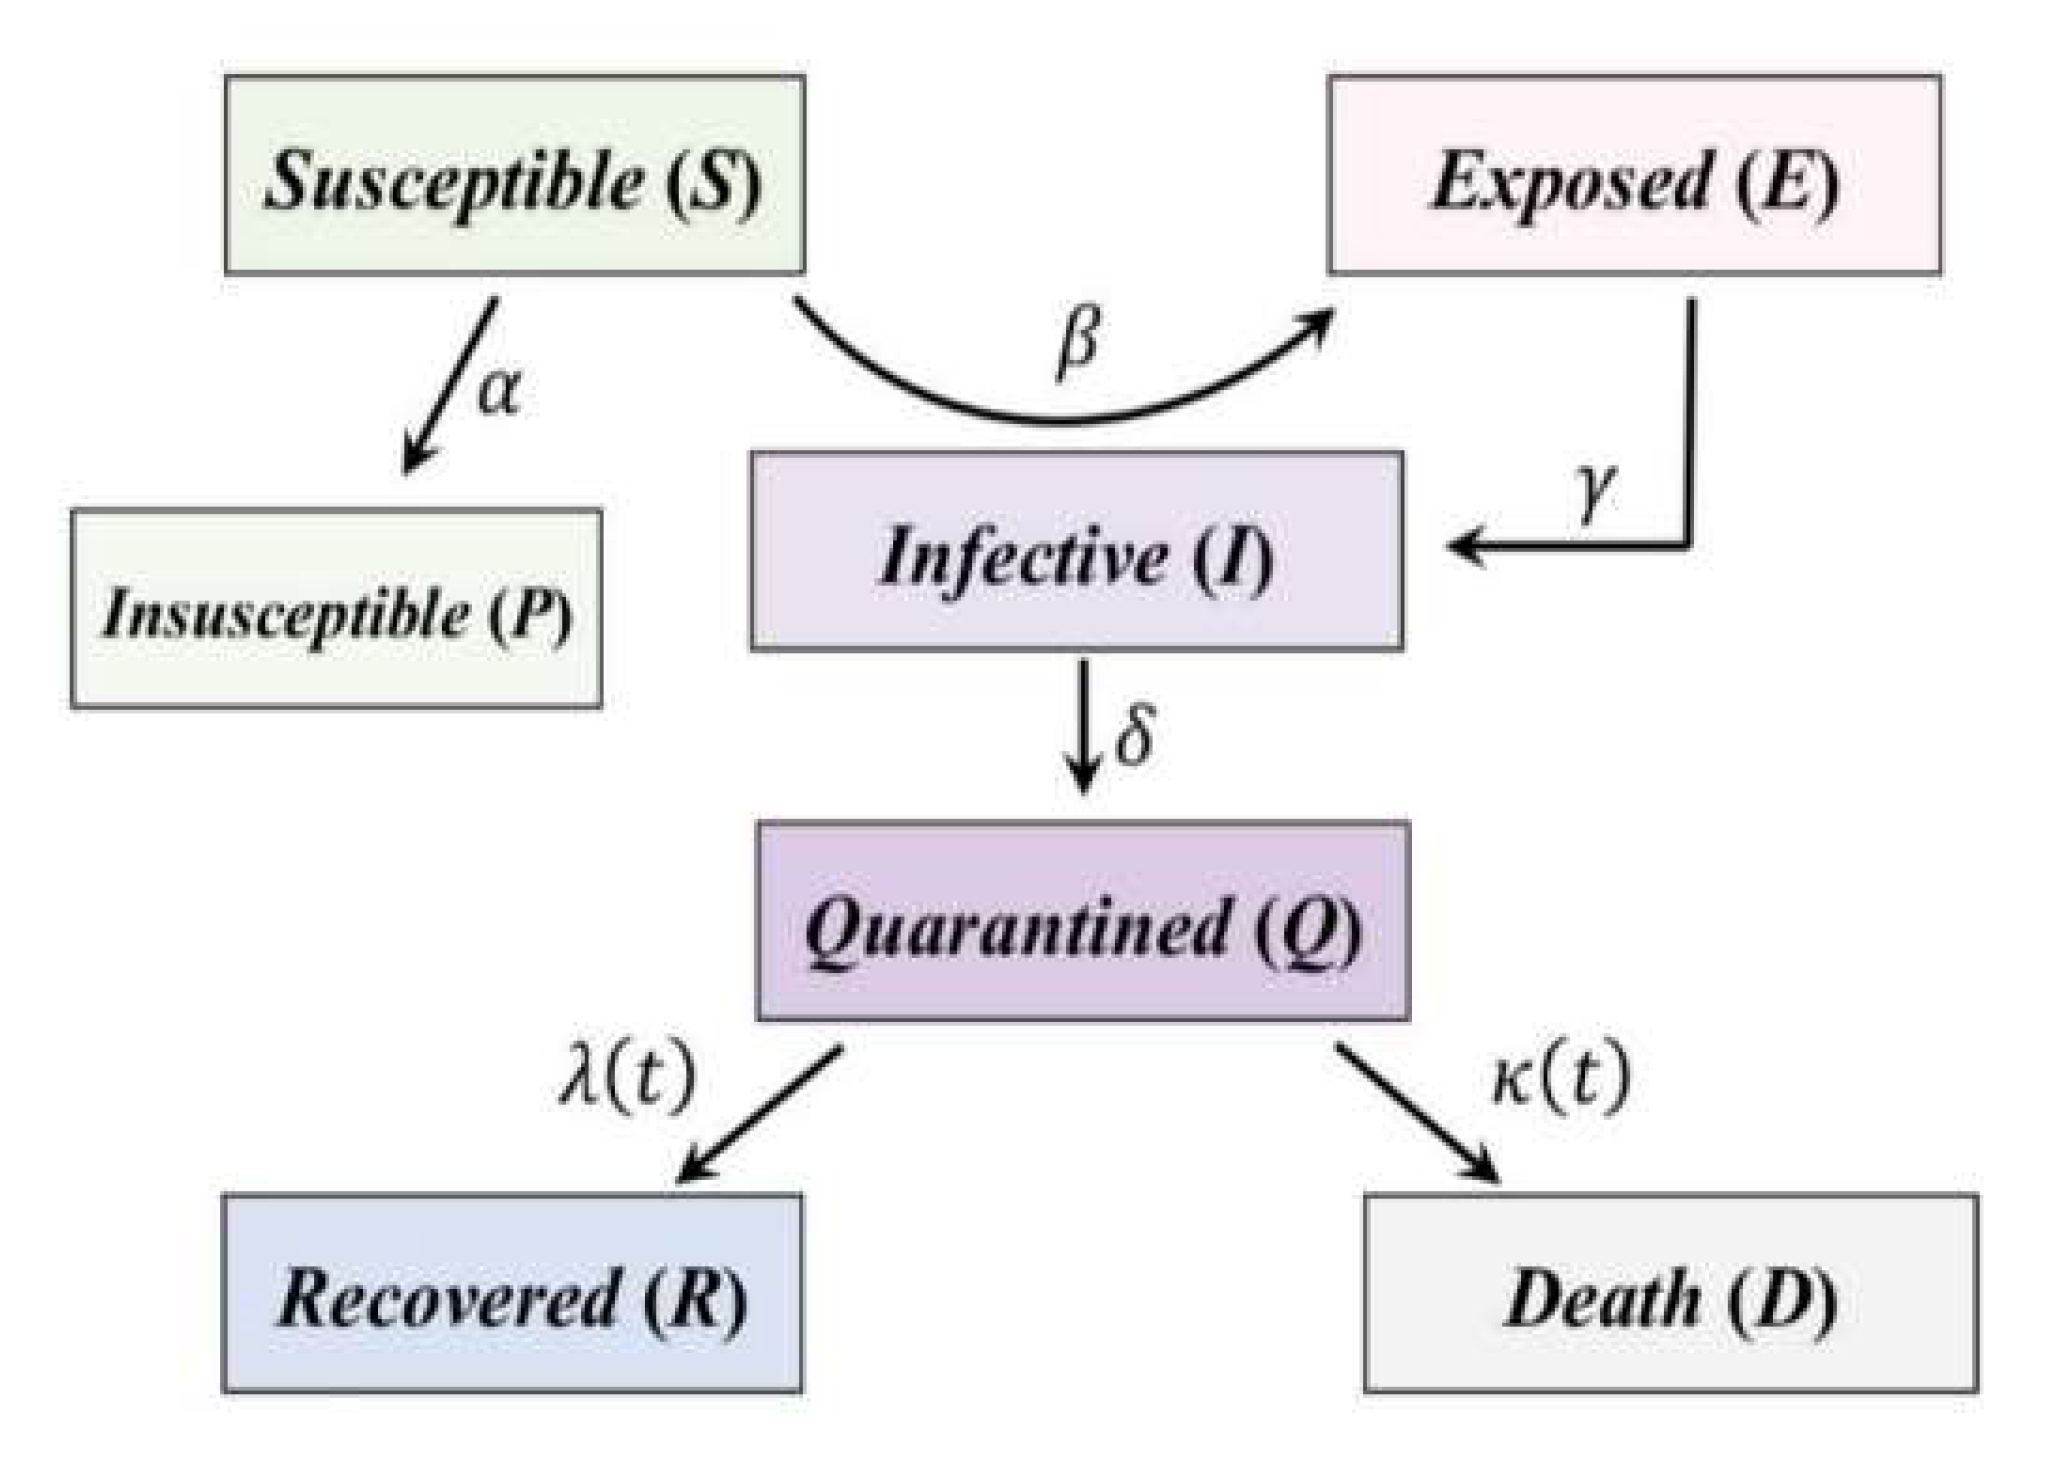
\includegraphics[width=\linewidth]{img/ijerph-17-03535-g001.png}
    \caption{Esempio di modello SEIR preso dall'articolo \cite{ijerph17103535}}
    \label{fig:SEIR_model}
\end{figure}

Il motivo per cui viene utilizzato il modello SEIR come base è perchè permette di 
modellare una caratteristica intrinseca di una malattia infettiva, ovvero 
il periodo di latenza che un individuo appena infettato ha prima di diventare 
infettivo a sua volta e mostrare i sintomi di infezione. Questo permette 
di osservare quanto le misure di sicurezza e prevenzione non farmaceutiche 
sono efficaci sulla popolazione tenendo in considerazione 
un tempo di ritardo intrinseco nel feedback tra l'attuamento delle 
misure di prevensione e i risultati positivi di queste ultime.

Una delle modifiche più utilizzate a questo modello è quella di avere un sistema 
ciclico, ovvero in cui gli individui che entrano nello stato R non diventano immuni 
alla malattia a tempo indefinito, ma perdono questa loro caratteristica di immunità
dopo un dato periodo di tempo. Questo permette di modellare con più accuratezza le malattie
infettive stagionali come ad esempio la comune influenza o il raffreddore, oppure 
mostrare l'andamento ad ondate di altre malattie che hanno la caratteristica di 
mutare molto velocemente, come è stato per il COVID-19 e le sue innumerevoli varianti.

Questa variante denominata SEIRS permette invece di osservare, non solo l'andamento e 
l'efficacia delle contromisure non farmaceutiche, ma anche di quelle
farmaceutiche, come ad esempio i vaccini; o più in generale l'andamento
della così detta immunità di gregge \cite{Bjornstad2020}. 

\newpage

\begin{figure}[h]
    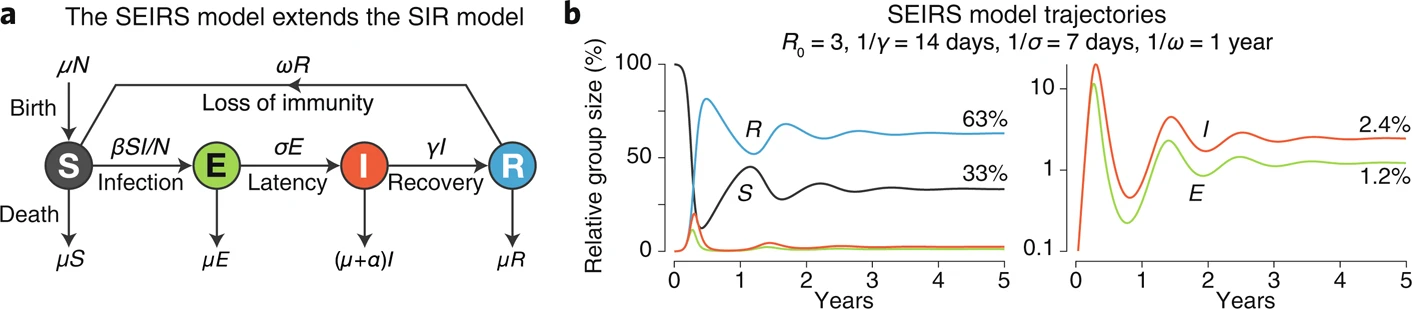
\includegraphics[width=\linewidth]{img/41592_2020_856_Fig1_HTML.png}
    \caption{Modello SEIRS preso dall'articolo \cite{Bjornstad2020}}
    \label{fig:SEIRS_model}
\end{figure}

Rimanendo sull'idea di voler analizzare l'efficacia di un vaccino, una
modifica comune al modello SEIR è quella legata all'aggiunta dello stato V,
Vaccinated, come stato esplicito oppure oppure implicito al modello. Questa 
variazione permette di modellallare con più attenzione l'efficacia di un 
vaccino una volta introdotto all'interno della popolazione, 
ma più in generale permette di osservare l'efficacia di una politica di vaccinazione 
in relazione al numero di vaccinazioni effettuate in un determinato periodo di tempo.
Questo viene solitamente affiancato con un modello ciclico, così da poter
osservare come bisogna modificare le proprie politiche vaccinali in vista
di ondate cicliche più o meno intense di infezioni.

\begin{figure}[h]
    \begin{center}
        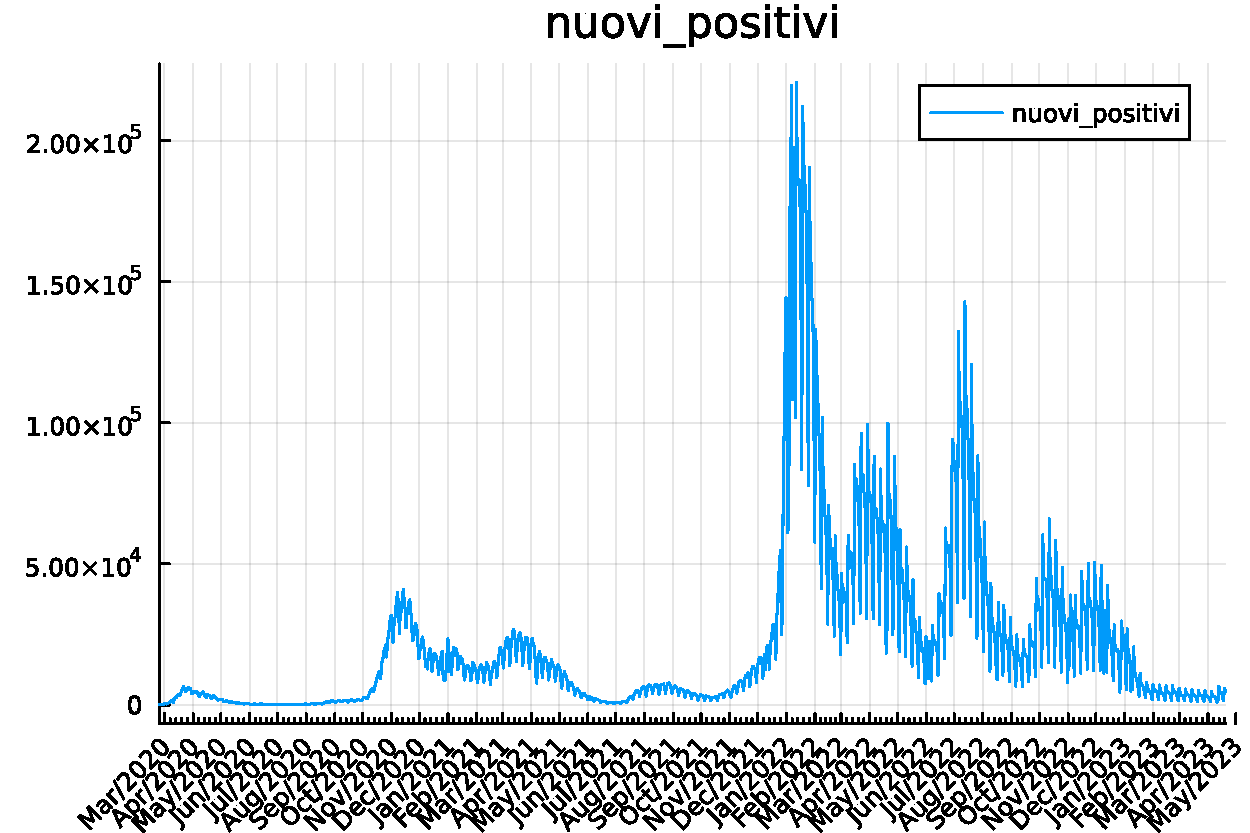
\includegraphics[scale=0.6]{img/nuovi_positivi_2023-04-21.pdf}
        \caption{Esempio di ondate di infettività. Dati del Dipartimento di Protezione Civile Italiana}
        \label{fig:DPC_new_positive}
    \end{center}
\end{figure}

Ai fini pratici di una simulazione avere uno stato esplicitamente definito
oppure ricavabile dalle probabilità di transizione degli altri stati 
è pressocchè indifferente, e potrebbe essere richiesta una diferenziazione
solamente in caso in cui si avrebbe una differenza sostanziale tra lo stato
R e V, ad esempio in termini di protezione dalla malattia, durata immunità etc... .

\begin{figure}[h]
    \begin{center}
        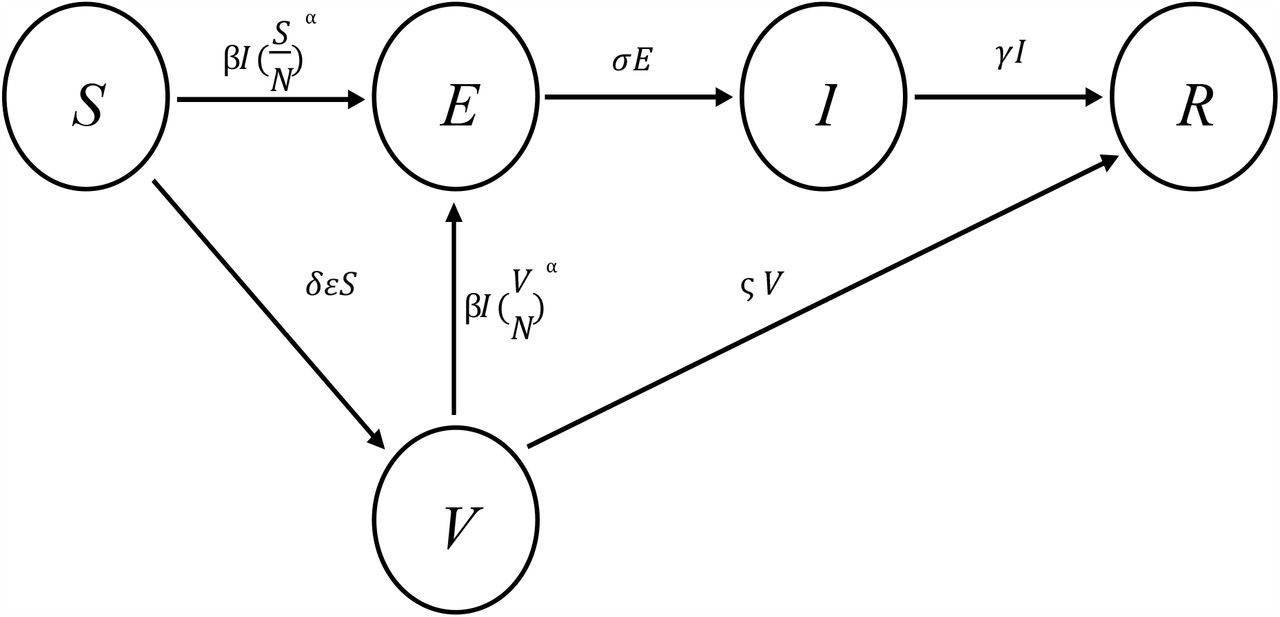
\includegraphics[scale=1.2]{img/seirv_explicit.jpg}
        \caption{Esempio di modello SEIRV con stato esplicito per la condizione V}
        \label{fig:SEIRV_explicit}
    \end{center}
\end{figure}

\begin{figure}[h]
    \begin{center}
        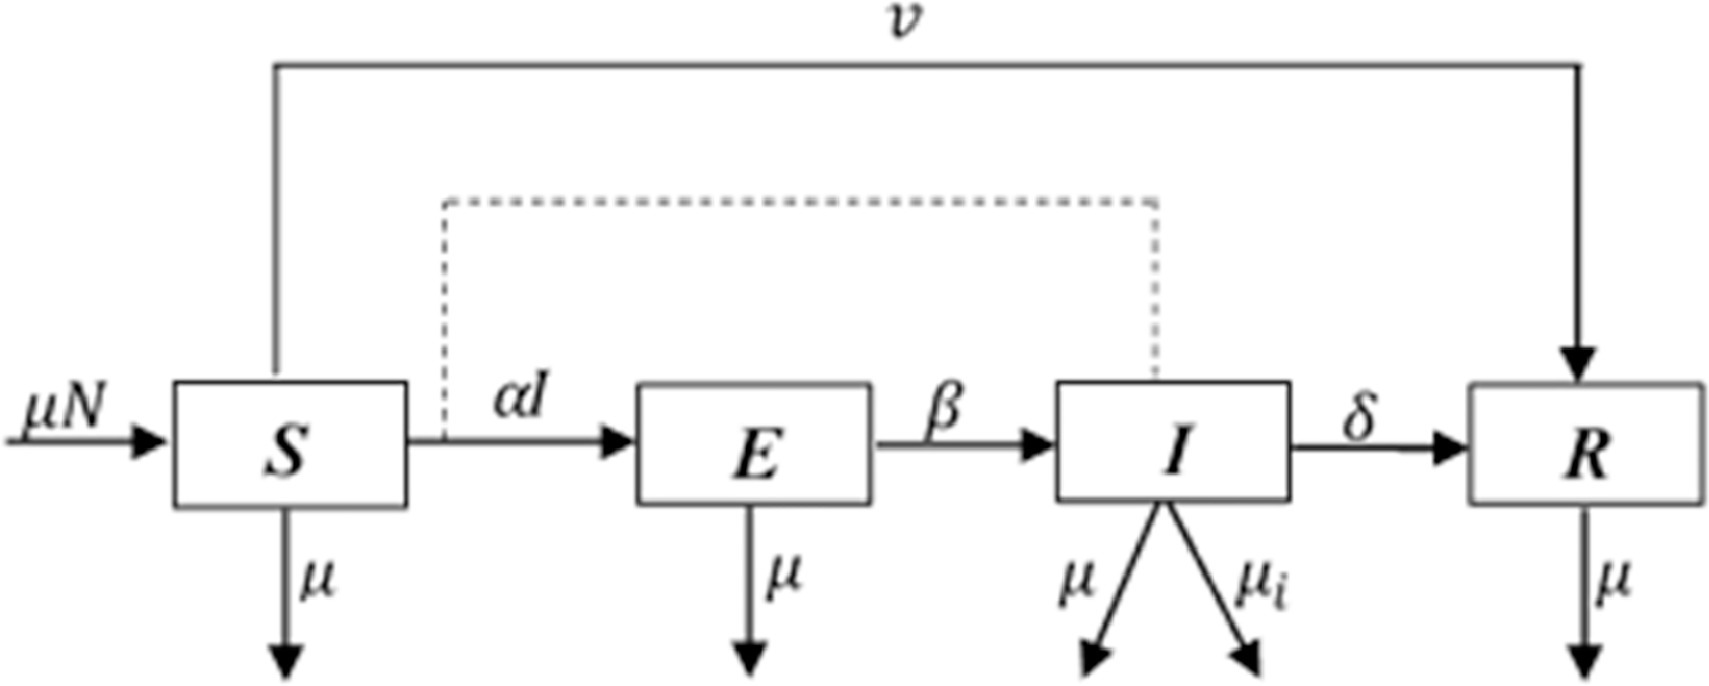
\includegraphics[scale=1.3]{img/seirv_implicit.jpg}
        \caption{Esempio di modello SEIRV con stato implicito per la condizione V}
        \label{fig:SEIRV_implicito}
    \end{center}
\end{figure}

Non essendoci un numero massimo di stati, e quindi di equazioni, utilizzabili
all'interno del modello, ogni individuo è libero di definire un numero
di equazioni arbitrario che rispecchia la sua idea di modellazione del 
sistema. Ne è un esempio il modello riportato in \cite{Giordano2020}.

Come precedentemente introdotto esistono due grandi famiglie di modelli
per la simulazione, e sono rispettivamente la famiglia di modelli deterministici
e quella di modelli stocastici.

\subsubsection{Modelli Deterministici}
Descrizione dei modelli di tipo deterministico con l'utilizzo delle ODE
Pro e Contro utilizzo modelli deterministici

\subsubsection{Modelli Stocastici}
Descrizione dei modelli di tipo stocastico con l'utilizzo delle SDE
Pro e Contro utilizzo modelli stocastici